\chapter{Einleitung}
Die graphische Darstellung von Daten, das Diagramm, ist von grosser Bedeutung für die Gesellschaft. Man findet Diagramme überall: In etlichen Wissenschaften, wo sie nicht wegzudenken sind, in jeglichen Industrien, in Zeitungen, in Werbungen.

Das Ziel eines Diagramms ist die Vermittlung von Zusammenhängen und Informationen des dargestellten Datensatzes. Der Leser sollte sich mit den Daten auseinandersetzen können, ohne die Rohdaten (die gesammelten Daten, die in dem Diagramm dargestellt werden) betrachten zu müssen. Je nachdem wie das Diagramm graphisch umgesetzt wird, können verschiedene Zusammenhänge und Informationen des Datensatzes hervorgehoben oder in den Hintergrund gestellt werden, was einen Einfluss auf die Vermittlung hat.

Im Informationszeitalter sind Daten von grosser Bedeutung, der Datenfluss vergrössert sich ständig. Um Daten darstellen zu können, müssen sie zuerst gesammelt, sortiert und formatiert werden, bevor mit der Auswertung begonnen werden kann. Das Sammeln von Daten stellt oftmals keine besondere Schwierigkeit dar, das Auswerten, Darstellen und Interpretieren ist eine Herausforderung.

Konventionell werden Diagramme in Zeitungen, Artikeln abgedruckt. Der Autor trifft Entscheidungen, wie die Daten in graphischer Form dargestellt werden und erstellt auf Basis dieser ein Diagramm. Nach dem Druck kann es vom Leser betrachtet werden, jedoch kann dieser die Darstellung nicht mehr verändern, das Diagramm ist statisch. Er hat darum keinen Einfluss, wie die Daten in diesem \textbf{statischen Diagramm} dargestellt und an ihn vermittelt werden.

Durch das Aufkommen von modernen Computern, Smartphones haben sich die Möglichkeiten zur Darstellung erweitert: Dem Nutzer ist es möglich, mit dem Diagramm zu interagieren. Man findet unter anderem in Online-Zeitschriften solche \textbf{dynamischen Diagramme}, welche Daten darstellen, die mit dem Artikel zu tun haben und interaktiv vom Nutzer bedient werden können. Die Abbildungen \ref{fig:nytimes-taxes} und \ref{fig:nytimes-realestate} demonstrieren, wie das Potential der Interaktion auf eine interessante Weise ausgenutzt werden kann.

In der Abbildung \ref{fig:nytimes-taxes} ist ein Blasendiagramm dargestellt. Jede Blase stellt eine Firma dar, je nach Börsenwert ist die Blase unterschiedlich gross. Die Firmen sind in horizontaler Richtung nach ihrem Steuertarif geordnet, die verschiedenen Farben stellen die jeweilige Industrie, in der die Firma tätig ist, dar. Wenn die Maus über die Blase fährt, wird ein \textit{Popup} sichtbar, das weitere Informationen zu der Firma anzeigt wie der exakte Steuertarif, die absolute Menge an Steuern, die bezahlt wurden oder der Umsatz der Firma.

\begin{figure}[!htbp]
	\centering
	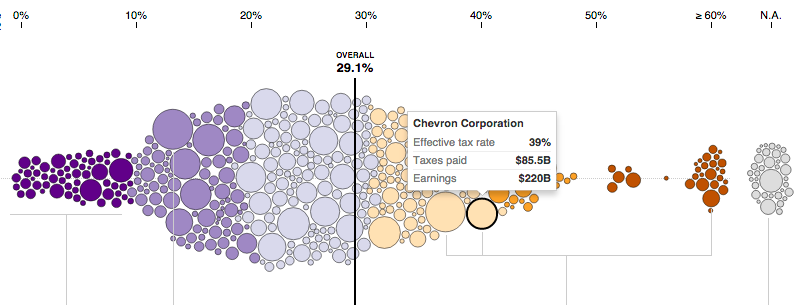
\includegraphics[width=\linewidth]{images/nytimes-taxes-zugeschnitten}
	\caption[Blasendiagramm in der New York Times]{Ein Blasendiagramm, das Steuerabgaben und Steuersätze von US-Firmen darstellt. \cite{nytimes-taxes}}
	\label{fig:nytimes-taxes}
\end{figure}

Die Webseite in Abbildung \ref{fig:nytimes-realestate} berechnet anhand von vom Benutzer festgelegten Faktoren, ob der Kauf eines Hauses profitabler wäre als die Miete. Es sind Faktoren vorhanden wie der Zinssatz, die Entwicklung der Miete und der Wert des Hauses, der Steuersatz für Grundstücke, die Inflationsrate. Die verschiedenen Faktoren kann der Benutzer durch einen \textit{Slider} anpassen. Dabei kann er durch die Höhe der Balken über dem Slider sehen, wie sich der Faktor auf das Resultat auswirkt (ob der Kauf oder die Miete profitabler wäre). Beim verschieben des Sliders wird das Ergebnis automatisch aktualisiert, so sieht der Nutzer den Zusammenhang der Faktoren und der Berechnung.

\begin{figure}[!htbp]
	\centering
	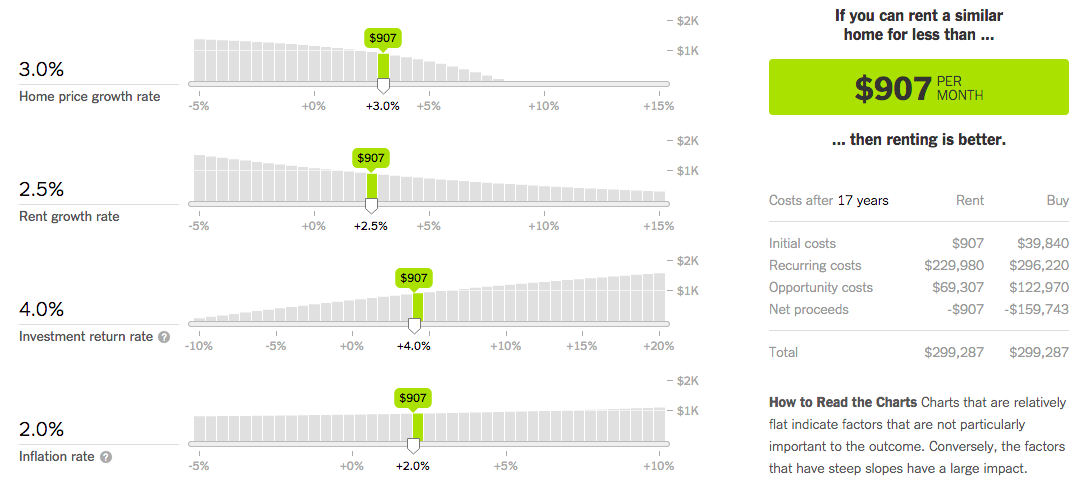
\includegraphics[width=\linewidth]{images/nytimes-realestate-zugeschnitten}
	\caption[Interaktives Diagramm in der New York Times]{Interaktives Diagramm mit verstellbaren Reglern, das die Profitabilität des Kaufs eines Hauses darstellt. \cite{nytimes-realestate}}
	\label{fig:nytimes-realestate}
\end{figure}

Diese Maturaarbeit wurde von dem Artikel \textit{The Eyes Have It: A Task by Data Type for Information Visualizations} von B. Shneidermann \cite{shneiderman} inspiriert. Der Artikel untersucht, wie ein Benutzer eine Programmoberfläche wahrnimmt und auf welche Weise er mit ihr interagiert. Auch beschreibt der Artikel, wie die Oberfläche aufgebaut sein sollte, damit der Benutzer sich im Programm orientieren kann, die Programmlogik versteht und es ohne grossen Aufwand bedienen kann. In dem Artikel stellte der zudem das \textit{Mantra der Informationsvisualisierung (Information-Seeking Mantra)} auf, das beschreibt, wie der Benutzer typischerweise mit einer Oberfläche interagiert: Überblick zuerst, Zoomen und Filtern, als letztes Details auf Abruf \cite{shneiderman}.

An den Diagrammen in \ref{fig:nytimes-taxes} und \ref{fig:nytimes-realestate} kann man den Vorteil von dynamischen Diagrammen gut demonstrieren: In \ref{fig:nytimes-taxes} wird der dritte Teil der Mantra der Informationsvisualisierung angewendet, Details auf Abruf: Der Tooltip zusätzliche Informationen einer angewählten Firma an. Wegen Platzmangel wäre es nicht möglich gewesen, die gesamte Information aller Firmen in einem statischen Diagramm darzustellen.

In \ref{fig:nytimes-realestate} verändern sich die einzelnen Diagramme je nach Einstellung der Faktoren. Diese Verhaltensweise ist nicht umzusetzen in einem statischen Diagramm.

Die von Shneidermann beschriebenen Prinzipien für das Design von Benutzeroberflächen werden in dieser Arbeit berücksichtigt. Es werden interaktive, dynamische Diagramme entwickelt, die den Informationsertrag des Nutzers verbessern sollten. Er sollte sich mit den Daten effizienter auseinandersetzen können, besser verstehen und Spass an der Erkundung des Datensatzes haben \cite{shneiderman}.

\section{Ziel dieser Arbeit}

<beschreiben was man überhaupt machen will. dynamische diagramme entwickeln, die - für den nutzer ansprechend sind und der nutzer gut versteht und einen effizienteren informationsertrag daraus nehmen kann und komplikationslos mit der applikation interagieren kann und spass macht>

\section{Wahl des Diagrammtyps}

Es gibt sehr viele Arten von Diagrammen, welche sich unterschiedlich für verschiedene Datentypen eignen. <beispiele pie diagramme und so?> Diese Arbeit beschränkt sich auf einen Diagrammtyp, das Streudiagramm. Das Streudiagramm wird in der Wissenschaft als auch in anderen Medien oft verwendet. Es stellt beobachtete Wertepaare zweier Merkmale dar. Diese zwei Werte werden als Punkte in ein kartesisches Koordinatensystem eingetragen, welches zwei- oder mehrdimensional sein kann. Dadurch entsteht eine Menge vom Punkten. In der Praxis, falls ein Verlauf von Werten, zum Beispiel über eine Zeit, dargestellt werden will, werden die Punkte oft nicht gezeichnet und durch eine Linie verbunden.

Die Beschränkung der Arbeit auf ein einzigen Diagrammtyp ermöglicht, dass man auf sehr spezifische Aspekte des Arbeitsproduktes eingehen kann und nicht die Untersuchung generell formulieren muss.

\section{Technologie}

Die interaktiven Diagramme werden in der Praxis fast ausschliesslich für den Web-Browser entwickelt, wie auch in dieser Arbeit. Technologien wie HTML (für den Inhalt), CSS (für das Aussehen), SVG (für Vektorgrafiken), JavaScript (für die Berechnung) werden verwendet, diese ermöglichen die dynamische Manipulation durch den Nutzer. Der Prozess der Entwicklung in diesen Technologien wird im Kapitel \ref{chapter:praktischer_teil} dokumentiert.
